\documentclass[aspectratio=169]{beamer}
\beamertemplatenavigationsymbolsempty
\usetheme{Boadilla}
\usepackage{textpos} % package for the positioning
\usepackage{enumitem}
\usepackage{amsmath,amsfonts,amssymb}

\usepackage{listings}
\usepackage{xcolor}

% Define color values for the theme
\definecolor{backcolour}{rgb}{0.97, 0.97, 1.0}    % Light purple background
\definecolor{codegreen}{rgb}{0.0, 0.6, 0.0}       % Green for comments
\definecolor{codegray}{rgb}{0.5, 0.5, 0.5}        % Gray for line numbers
\definecolor{codepurple}{rgb}{0.58, 0.0, 0.83}    % Purple for strings
\definecolor{keywordcolor}{rgb}{0.5, 0.0, 0.5}    % Dark purple for keywords

% Define the style for the listings
\lstdefinestyle{mystyle}{
    backgroundcolor=\color{backcolour},
    commentstyle=\color{codegreen},
    keywordstyle=\color{keywordcolor},
    numberstyle=\tiny\color{codegray},
    stringstyle=\color{codepurple},
    basicstyle=\ttfamily\footnotesize,
    breakatwhitespace=false,
    breaklines=true,
    captionpos=b,
    keepspaces=true,
    numbers=left,
    numbersep=5pt,
    showspaces=false,
    showstringspaces=false,
    showtabs=false,
    tabsize=2
}

\lstset{style=mystyle}

\definecolor{uwopurple}{RGB}{79,38,131} % official purple color for uwo


\title{Foundations of Quantum Computing}
\author[]{Zyad Altahan (50238152) \and \AA{AAAAAAAAAA AAAAAAA}{6} (\AA{AAAAAAAA}{10}) \and Tobias Mette (3105540) \and Aksa Aksa (50146305) \and Mohamed Sonbol (50262724)}
\institute[]{Department of Computer Science \\ University of Bonn}
\date{\today}

\usepackage[listings,many]{tcolorbox}
\makeatletter
\newtcblisting{mylisting}{
  listing only,
  breakable, enhanced jigsaw,
  listing engine=listings,
  colback=gray!20,
  listing options={
    language=python,
    keywordstyle=\color{blue},
    basicstyle=\ttfamily,
    stringstyle=\color{ForestGreen},
    commentstyle=\color{gray},
    ndkeywordstyle={\color{orange}},
    identifierstyle=\color{black},
    numbers=none,
    showstringspaces=false,
    aboveskip={0\p@ \@plus 6\p@}, belowskip={0\p@ \@plus 6\p@},
    columns=fullflexible, keepspaces=true,
    breaklines=true, breakatwhitespace=true,
    extendedchars=false,
    inputencoding=utf8,
    upquote=true,
    xleftmargin=-25pt,
  }
}
\makeatother

% set color
\setbeamercolor{title in head/foot}{bg=white}
\setbeamercolor{author in head/foot}{bg=white}
\setbeamercolor{date in head/foot}{fg=uwopurple}
\setbeamercolor{date in head/foot}{bg=white}
\setbeamercolor{title}{fg=uwopurple}
\setbeamerfont{title}{series=\bfseries}
\setbeamercolor{frametitle}{fg=uwopurple}
\setbeamerfont{frametitle}{series=\bfseries}
\setbeamercolor{block title}{bg=uwopurple!30,fg=black}
\setbeamercolor{item}{fg=uwopurple}
\setbeamercolor{caption name}{fg=uwopurple!70!}
\usefonttheme[onlymath]{serif}


\graphicspath{{./} {img/}}
\begin{document}


\begin{frame}
    \titlepage
    \begin{textblock*}{8cm}(5.0cm,-7.0cm)
        {\large \color{uwopurple}\hspace{0.66cm} \textbf{Exercise Sheet 02}} % Change the lecture # right here!
    \end{textblock*}
\end{frame}


\begin{frame}[fragile]{Task 2.1: Hadamard transforms}

\textbf{a)} We calculated the Hadamard matrix recursively using the Kronecker product from NumPy, i.e., \texttt{np.kron(hadamard\_matrix(1), hadamard\_matrix(n-1))}.

\vspace{1em}

\textbf{b)} We calculated the values $f_{110}$ and $f_{126}$ by taking the inverse of the Hadamard matrix $H_3$, for example, \texttt{hadamard110 = np.linalg.inv(hadamard\_matrix(3)) * rule110}.
\end{frame}

\begin{frame}[fragile]{Task 2.1: Hadamard transforms}

{\footnotesize
\textbf{c and d)} From the results, we can see that \( H_n^\dagger H_n = I \), confirming that the normalized Hadamard matrix \( H_n \) is orthogonal. This result implies that the rows and columns of \( H_n \) are orthonormal, meaning each row and column has unit length and is orthogonal to all others. Consequently, the rows (or columns) of \( H_n \) form an orthonormal basis for \( \mathbb{R}^{2^n} \), allowing any vector in this space to be represented uniquely as a combination of these basis vectors. The orthogonality also makes \( H_n \) invertible, so any vector \( f \) can be recovered from its Hadamard transform \( w \), guaranteeing that every \( 2^n \)-dimensional vector has a Hadamard transform. This orthonormal basis guarantees that every \( 2^n \)-dimensional vector has a unique Hadamard transform.

Thus, we don’t need to calculate an inverse explicitly; we can directly solve for $w_{110}$ and $w_{126}$ by taking advantage of this orthogonality for part d.
}

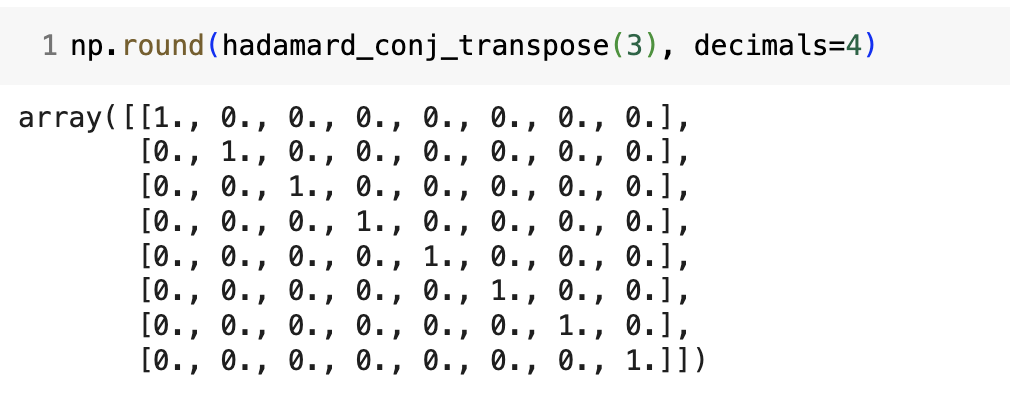
\includegraphics[width=08cm, height=04cm]{2.1_c_result.png}

\end{frame}


\begin{frame}[fragile]{Task 2.2: fourier transforms}
\textbf{a)} We were asked to create a function that creates the corresponding Fourier matrix given by this formula $F_n = \frac{1}{\sqrt{2^n}} \exp\left(i \frac{2 \pi j k}{2^n}\right)$
\begin{lstlisting}[language=Python]
def fourier_matrix(n):
    size = 2**n
    Js = np.stack([np.arange(size)]*size, axis=1)
    Ks = np.stack([np.arange(size)]*size, axis=0)

    return (1 / np.sqrt(size)) * np.exp(1j*2*np.pi*Js*Ks / size)
\end{lstlisting}
\end{frame}

\begin{frame}[fragile]{Task 2.2: fourier transforms}
\textbf{b)} We were asked to calculate the Fourier transforms of rules 110 and 126 given by this formula $f_{rule} = F_3 w_{rule}$ we should solve for $w_{rule}$ which we did by multiplying $F_3^{-1}$ with $f_{rule}$ to get the corresponding $w_{rule}$

\[
\begin{array}{c@{\hspace{1cm}}c}  % Adds horizontal space between matrices
    \text{$w_{110}$} & \text{$w_{126}$} \\[0.3em] % Titles for each matrix
    \begin{bmatrix}
         1.7678 + 0j \\
        -0.25 + 0.25j \\
        -0.7071 + 0.3536j \\
         0.25 + 0.25j \\
        -0.3536 + 0j \\
         0.25 - 0.25j \\
        -0.7071 - 0.3536j \\
        -0.25 - 0.25j
    \end{bmatrix}
    &
    \begin{bmatrix}
         2.1213 + 0j \\
        -0.6036 + 0.25j \\
        -0.3536 + 0.3536j \\
        -0.1036 + 0.25j \\
         0 - 0j \\
        -0.1036 - 0.25j \\
        -0.3536 - 0.3536j \\
        -0.6036 - 0.25j
    \end{bmatrix}
\end{array}
\]

\end{frame}

\begin{frame}[fragile]{Task 2.2: fourier transforms}
\textbf{c)} We were asked to reproduce our results by using function fft in module numpy.fft and choosing a suitable norm value which we did by using norm = "ortho" which gave identical results.

\begin{lstlisting}[language=Python]
np.fft.fft(rule110,norm='ortho')
\end{lstlisting}

\textbf{d)} We were asked to Compute the expression $F_n^{\dagger} Fn$ for several choices of n and discuss what we observe. These resulted in the identity which implies that the columns of $F_n$ are orthonormal, and $F_n$ is unitary. The unitarity of
$F_n$
  implies that every
$2^n$-dimensional vector has a Fourier transform.

\begin{lstlisting}[language=Python]
np.matmul(fourier_matrix(n).conj().T, fourier_matrix(n))
\end{lstlisting}

\end{frame}


\begin{frame}{Task 2.3a: vector spaces over Boolean rings}

\textbf{t.s.:} $(\mathbb{B}^n, \oplus, \cdot )$ is a \textbf{vector space} for $n>1\in \mathbb{N}$ over $\mathcal{R} = (\mathbb{B}, \oplus, \cdot )$\newline
Let $a, b, c \in \mathcal{R}$ and $u, v, w \in \mathbb{B}^n$, we have to show:\newline

\underline{\textbf{1) Associativity $(``\oplus")$}:} $u \oplus (v \oplus w) = (u \oplus v) \oplus w$\newline

$\bullet$ $a, b\in \mathcal{R} \Rightarrow a \oplus b \in \mathcal{R}$\newline

$\bullet$ the boolean XOR $(``\oplus")$ is associative:
$a\oplus (b \oplus c) = (a \oplus b) \oplus c$\newline

$\bullet$ $u \oplus (v \oplus w)$ = $u$ $\oplus
\begin{pmatrix}
v_1 \oplus w_1\\
\vdots\\
v_n \oplus w_n\\
\end{pmatrix} =
\begin{pmatrix}
u_1 \oplus (v_1 \oplus w_1)\\
\vdots\\
u_n \oplus (v_n \oplus w_n)\\
\end{pmatrix} =
\begin{pmatrix}
(u_1 \oplus v_1) \oplus w_1\\
\vdots\\
(u_n \oplus v_n) \oplus w_n\\
\end{pmatrix} = (u \oplus v) \oplus w$
\end{frame}

\begin{frame}{Task 2.3a: vector spaces over Boolean rings}
\underline{\textbf{2) Commutativity $(``\oplus")$}:} $u \oplus v = v \oplus u$\newline

$\bullet$ the boolean XOR $(``\oplus")$ is commutative: $a \oplus b = b \oplus a$\newline

$\bullet$ $u \oplus v =
\begin{pmatrix}
u_1 \oplus v_1\\
\vdots\\
u_n \oplus v_n\\
\end{pmatrix} =
\begin{pmatrix}
v_1 \oplus u_1\\
\vdots\\
v_n \oplus u_n\\
\end{pmatrix} = v \oplus u$\newline

\underline{\textbf{3) Identity Element $(``\oplus")$}:} $\mathcal{O} \in \mathbb{B}^n \Rightarrow v + \mathcal{O} = v$\newline

$\bullet$ $\mathcal{O} =
\begin{pmatrix}
0\\
\vdots\\
0\\
\end{pmatrix} \Rightarrow v + \mathcal{O} =
\begin{pmatrix}
v_1 \oplus 0\\
\vdots\\
v_n \oplus 0\\
\end{pmatrix} = v$\newline
\end{frame}

\begin{frame}{Task 2.3a: vector spaces over Boolean rings}

\underline{\textbf{4) Inverse Element $(``\oplus")$}:} $v \in \mathbb{B}^n \Rightarrow - v \in \mathbb{B}^n$: $v \oplus (- v) = 0$.\newline
$\bullet$ Define $- v$ as $v \Rightarrow v \oplus (- v) = v \oplus v = 0$\newline

\underline{\textbf{5) Compatibility of scalar multiplication with field multiplication $(``\cdot")$}:} $a(bv) = (ab)v$.\newline
$\bullet$ $a, b \in \mathcal{R} \Rightarrow a \cdot b \in \mathcal{R}$\newline
$\bullet$ field multiplication is associative: $a \cdot (b \cdot c) = (a \cdot b) \cdot c$\newline

$\bullet$ $a(bv) = a \cdot
\begin{pmatrix}
b \cdot v_1\\
\vdots\\
b \cdot v_n\\
\end{pmatrix} =
\begin{pmatrix}
a \cdot (b \cdot v_1)\\
\vdots\\
a \cdot (b \cdot v_n)\\
\end{pmatrix} =
\begin{pmatrix}
(a \cdot b) \cdot v_1\\
\vdots\\
(a \cdot b) \cdot v_n\\
\end{pmatrix} = (ab)v$\newline

\underline{\textbf{6) Identity Element of scalar multiplication $(``\cdot")$}:} $1 \in \mathcal{R} \Rightarrow 1 \cdot v = v$.\newline

$\bullet$ $1 \cdot v =
\begin{pmatrix}
1 \cdot v_1\\
\vdots\\
1 \cdot v_n\\
\end{pmatrix} =
\begin{pmatrix}
v_1\\
\vdots\\
v_n\\
\end{pmatrix} = v$

\end{frame}
\begin{frame}{Task 2.3a: vector spaces over Boolean rings}

\underline{\textbf{7) Distributivity of scalar mult. with resp. to vector addition $(``\cdot")$}:} $a(u \oplus v) = au \oplus av$\newline

$\bullet$ field multiplication is distributive with resp. to $(``\oplus")$: $a\cdot (b \oplus c) = a \cdot b \oplus a \cdot c$\newline

$\bullet$ $a(u \oplus v) = a \cdot
\begin{pmatrix}
u_1 \oplus v_1\\
\vdots\\
u_n \oplus v_n\\
\end{pmatrix} =
\begin{pmatrix}
a \cdot (u_1 \oplus v_1)\\
\vdots\\
a \cdot (u_n \oplus v_n)\\
\end{pmatrix} =
\begin{pmatrix}
a \cdot u_1 \oplus a \cdot v_1\\
\vdots\\
a \cdot u_n \oplus a \cdot v_n\\
\end{pmatrix} = au \oplus av$\newline


\underline{\textbf{8) Distributivity of scalar mult. with resp. to field addition$(``\cdot")$}:} $(a \oplus b)v = av \oplus bv$\newline

$\bullet$ $(a \oplus b)\cdot v =
\begin{pmatrix}
(a \oplus b) \cdot v_1\\
\vdots\\
(a \oplus b) \cdot v_n\\
\end{pmatrix} =
\begin{pmatrix}
a \cdot v_1 \oplus b \cdot v_1\\
\vdots\\
a \cdot v_n \oplus b \cdot v_n\\
\end{pmatrix} = av \oplus bv$\newline

All 8 conditions are fulfilled.\newline
$\Rightarrow (\mathbb{B}^n, \oplus, \cdot )$ is a \textbf{vector space} for $n>1\in \mathbb{N}$ over $\mathcal{R} = (\mathbb{B}, \oplus, \cdot )$
\end{frame}







\begin{frame}{Task 2.3b: vector spaces over Boolean rings}

\textbf{t.s.:} $\langle x, y\rangle = \sum^{n}_{j=1} x_j \cdot y_j$  is an \textbf{inner product} for the vector space $(\mathbb{B}^n, \oplus, \cdot )$.\newline
We have to show:\newline

\textbf{1) Conjugate symmetry}: $\langle x, y\rangle = \overline{\langle y, x\rangle}$\newline
$\bullet$ $\langle x, y\rangle = \sum^{n}_{j=1} x_j \cdot y_j = x_1 \cdot y_1 + \cdot \cdot \cdot + x_n \cdot y_n = y_1 \cdot x_1 + \cdot \cdot \cdot + y_n \cdot x_n = \langle y, x\rangle$\newline
$\bullet$ $\langle y, x\rangle \in \mathbb{B}$ because $(``\cdot")$ and $(``+")$ are closed over $\mathbb{B}$\newline
$\bullet$ $\langle y, x\rangle \in \mathbb{B} \Rightarrow \overline{\langle y, x\rangle} = \langle y, x\rangle = \langle x, y\rangle$ because $\mathbb{B} \subset \mathbb{R}$\newline

\textbf{2) Linearity in first argument}: $\langle ax + by, z\rangle = a\langle x, z\rangle + b\langle y, z\rangle$\newline
$\bullet$ $\langle ax + by, z\rangle = \sum^{n}_{j=1} (ax_j + by_j) \cdot z_j = ax_1z_1 + by_1z_1 + \cdot \cdot \cdot + ax_nz_n + by_nz_n\newline
= ax_1z_1 + \cdot \cdot \cdot+ ax_nz_n + by_1z_1+ \cdot \cdot \cdot + by_nz_n\newline
= a\cdot \sum^{n}_{j=1} x_j \cdot z_j + b\cdot \sum^{n}_{j=1} y_j \cdot z_j = a\langle x, z\rangle + b\langle y, z\rangle$\newline

\end{frame}
\begin{frame}{Task 2.3b: vector spaces over Boolean rings}
\textbf{3) Positive-definiteness}: $\langle x,x\rangle \geq 0$ for all $x \in \mathbb{B}^n$ \textbf{and} $\langle x,x\rangle = 0 \Leftrightarrow x = \mathcal{O}$\newline

$\bullet$ $\langle x,x\rangle \geq 0$ holds because $x, y \in \mathbb{B}^n \Rightarrow \langle x,y\rangle \in \mathbb{B}=\{0, 1\}$\newline

$\bullet$ $x = \mathcal{O} \Rightarrow \langle x,x\rangle = \langle \mathcal{O},\mathcal{O}\rangle = \sum^{n}_{j=1} 0 \cdot 0 = 0 + \cdot \cdot \cdot + 0 = 0$ \newline

$\bullet$ $\langle x,x\rangle = 0 \Rightarrow \sum^{n}_{j=1} x_j \cdot x_j = x_1x_1 + \cdot \cdot \cdot + x_nx_n = 0 \Rightarrow x = \mathcal{O}$ \newline

$\Rightarrow \langle x, y\rangle$ is an inner product for the vector space $(\mathbb{B}^n, \oplus, \cdot )$.

\end{frame}

\begin{frame}{Task 2.4: Bool-Möbius transforms}
\textbf{a): Sierpiński Matrix Generation}\\
Generating a Sierpiński matrix \( S_n \) will be based on the formula: \( S_n = S_1 \otimes S_{n-1} \)\\
Using \( S_1 = \begin{bmatrix} 1 & 0 \\ 1 & 1 \end{bmatrix} \), which will be doneted as $sierpinski_1$.\\
The generation function \texttt{generate\_sierpinski\_matrix(n)} constructs \( S_n \) recursively by calling \texttt{np.kron($sierpinski_1$, generate\_sierpinski\_matrix(n-1))}, where \texttt{np.kron} is the the Kronecker product \( \otimes \).\\
The function will start from n and will reach the base case where $n = 1$. Then, it will return \( S_1\) and backtrack to build the matrix all the way up to \( S_{n-1}\) and finally multiply the result with \( S_1\).

\end{frame}

\begin{frame}{Task 2.4: Bool-Möbius transforms}
\textbf{b): Squaring Sierpiński Matrix \( S_n^2 = S_n \cdot S_n \)}\\
Using Boolean Matrix multiplication function: \texttt{boolean\_matrix\_multiply}, which iterates through elements of two matrices \( A \) and \( B \) and computes the result by:
\begin{itemize}
    \item Initializing each entry in the result matrix to zero.
    \item Using AND to multiply corresponding elements and XOR to combine results in each row-column product.
\end{itemize}
It will provide the result of 2 Sierpinski matrix Boolean products \(S_n \cdot S_n\ = S_n^2 \).\\
\textbf{Obervation: }\\
By looking at the result of \( S_n^2 \) e.g. $n=2$\\ \( S_2^2
\begin{bmatrix}
1 & 0 & 0 & 0 \\
0 & 1 & 0 & 0 \\
0 & 0 & 1 & 0 \\
0 & 0 & 0 & 1 \\
\end{bmatrix}
\)\\
We find that \( S_n^2 = I_n \), which is the identity matrix $I_n$. This means that Sierpiński matrix
$S_n$ is its own inverse as \(S_n \cdot S_n = I_n \).
\end{frame}

\begin{frame}{Task 2.4: Bool-Möbius transforms}
\textbf{c): Bool-Mobius transforms of rules 110 and 126}\\
Using the above we can calculate the rules 110 and 126 by solving the equations \( f_{110} = S_3 \cdot w_{110} \) and \( f_{126} = S_3 \cdot w_{126} \), where \( S_3 \) is a 3-dimensional Sierpinski matrix. We create a boolean vector-matrix multiplication function similar to the matrix-matrix multiplication done in the previous step.
The outputs are \( f_{110} = [0 1 1 1 0 0 0 1] \) and \( f_{126} = [0 1 1 1 1 1 1 0] \) represent the inverse transforms for rules 110 and 126.

\end{frame}

\begin{frame}{Task 2.5: yet another feature transform}

\textbf{a) Binary solution}:
Compared to the previous feature transform, this one has the exact same ordering as binary counting. So we can use the binary representation matrix of integers in $[0,2^n)$ as a mask for the vector $\mathbf{x}$, and then compute the row-wise product. All this is very easily done in \texttt{numpy}.
\vspace{.6cm}

\textbf{b) Kronecker solution}:
By analogy with the recursive Kronecker-based definition given in task 2.1, we can construct our own definition, where $F_\mathbf{x}^{(n)}$ denotes the feature transform of the first $n$ bits of $\mathbf{x}$.
\begin{align*}
    F_\mathbf{x}^{(1)} &= \begin{bmatrix} 1 \\ x_1 \end{bmatrix} \\
    F_\mathbf{x}^{(n)} &= F_\mathbf{x}^{(n-1)} \otimes \begin{bmatrix} 1 \\ x_n \end{bmatrix}
\end{align*}
This recursion adds one bit to the resulting vector with each iteration, and doubles that vector in size.

\end{frame}


\end{document}
